\chapter{Theory}

\section{Modelling of light propagation in breast tissue}
Photon that propagates through tissue can be described by the radiative transport equation, and in the case of low absorption, can be approximated as a diffusive process. The derivation of the photon diffusion equation from the transport equation has its origin in nuclear transport theory \cite{Case1967}. For now we will simply state that in a homogenous media with low absorption and high scattering, the photon fluence rate
$\Phi({\bf r},t) \ (W/cm^{2})$ obeys the diffusion equation:
\begin{equation}
\label{DEtime}
\nabla\cdot ( D({\bf r}) \nabla \Phi({\bf r},t)) - v\mu_a({\bf r}) \Phi({\bf r},t) + v S({\bf r},t) = \frac{\partial \Phi({\bf r},t)}{\partial t}
\end{equation}
\noindent
where ${\bf r}$ is the position vector, $t$ is time, $v$ is the speed of light in the medium, $\mu_a({\bf r})\ (cm^{-1})$ is the absorption coefficient, $D(\vec{r})=\frac{v}{3(\mu_s^{\prime}({\bf r}))}$ is the diffusion coefficient constant where $\mu_s'({\bf r}) (cm^{-1})$ is the reduced scattering coefficient, and $S({\bf r},t)\ (W/cm^{3})$ is the source term. \\
For clarification, $\Phi$ is not fluence which is commonly defined as number per area ($m^{-2}$) or energy per area ($J/m^{2}$). In the frequency domain we modulate our point light source (which we can model with a delta function) which results in our source and detected signals having a DC and AC component. 
\begin{eqnarray}
\label{AC}
S({\bf r},t) & = & [S_{DC} + S_{AC}e^{-i\omega
  t}]\delta({\bf r}) \\
\Phi({\bf r},t) & = & \Phi({\bf r})_{DC} + \Phi({\bf r})_{AC}e^{-i\omega t}
\end{eqnarray}
\noindent
Focusing on just the AC component, the diffusion equation will become
\begin{equation}
\label{DE}
[-\nabla \cdot D({\bf r}) \nabla + v \mu_a({\bf r})-i\omega]\Phi_{AC}({\bf
  r},\omega)=vS_{AC}\delta({\bf r})
\end{equation}
\noindent
We will now solve for this equation analytically for the infinite, semi-infinite and slab geometries.

\subsection{Analytical Solutions}
In this section we will go over three analytical solutions to the photon diffusion equation. We will solve for the fluence rate $\Phi$ in the infinite, the semi-infinite, and the slab geometries in a homogeneous media. For the infinite medium, we will find the solution by solving the Green's function for the Helmholtz
equation. For the semi-infinite and slab problems we will use the method of images after determining the extrapolated boundary condition for the appropriate placement of our sources and sinks.
\subsubsection{Infinite Geometry}
We will go over two methods of solving for the infinite geometry. The first method will follow the solution from section 6.4 of Jackson's E\&M textbook \cite{JacksonEM}. We start with the diffusion equation in the frequency domain (Equation \ref{DE}). Assuming that we are working with in a homegeneous media, we can now say that $D$ is a constant. Dividing both sides by $D$ and defining a constant $k_0 = \frac{- c\mu_a + i\omega}{D}$, we get 
\begin{equation}
\label{DEHelm}
(\nabla^2+k_0^2)\Phi({\bf r})=-\frac{vS_{AC}}{D}\delta({\bf r})
\end{equation}
\noindent
Here we will define ${\bf r}$ the position vector a distance $r$ away from the source. In this form we see that the photon fluence rate $\Phi$ is the Green's function for the Helmholtz equation.
\begin{equation}
\label{greenHelm}
(\nabla^2+k_0^2)G({\bf r})=-\frac{vS_{AC}}{D}\delta({\bf r})
\end{equation}
\noindent
In the infinite medium, there are no boundary surfaces the Green's function is spherically symmetric and will depend only on $r={\bf r}$. The Laplace equation in spherical coordinates is then:
\begin{eqnarray}
\label{laplacian}
\nabla^2 & \equiv & \frac{1}{r}\frac{\partial^2}{\partial r^2}r 
+ \frac{1}{r^2\sin^2\theta}\frac{\partial^2}{\partial\phi^2}
+ \frac{1}{r^2\sin\theta}\frac{\partial}
{\partial\theta}\left(\sin\theta\frac{\partial}{\partial\theta}\right)
\nonumber \\
& = & \frac{1}{r}\frac{\partial^2}{\partial r^2}r
\end{eqnarray}
Then equation \ref{greenHelm} becomes
\begin{equation}
\label{greenHelmLaplace}
\frac{1}{r}\frac{\partial^2}{\partial r^2}rG(r) + k_0^2G(r) 
=-\frac{vS_{AC}}{D}\delta(r)
\end{equation}
\noindent
at every point except at ${\bf r} = 0$ the equation above becomes 
\begin{equation}
\label{greenHelmLaplaceHomog}
\frac{\partial^2}{\partial r^2}[rG(r)] + k_0^2[rG(r)] = 0
\end{equation}
\noindent
with the solution at every point except at $r = 0$ the equation above becomes 
\begin{equation}
\label{greenHelmLaplaceSoln1}
G(r) = \frac{A e^{ik_0r} + B e^{-ik_0r}}{r} = \frac{A e^{ik_0r}}{r}
\end{equation}
The first term of the Green's function is propagating away from the source while the second term converges, so we will only keep the first
term. We could also argue that as we move infinitely away from the source the Green's function needs to go to zero which would mean that $B=0$ by noting that $k_0$ is complex. \\
Now to solve for A, we go back to equation \ref{greenHelm}, we take a volume integral on both sides in the limit where $r \rightarrow 0$ where the delta function exists.
\begin{equation}
\label{greenHelmdelta}
\lim_{r\rightarrow 0}\int_V[\nabla^2G({\bf r})+k_0^2G({\bf r})]dV =
-\lim_{r\rightarrow 0}\int_V \frac{vS_{AC}}{D}\delta({\bf r})dV =-\frac{vS_{AC}}{D}
\end{equation}
\noindent
Looking at the second term on the LHS in spherical coordinates, we see that it goes to zero
\begin{equation}
\label{greenHelm2nd}
\lim_{r\rightarrow 0}\int_Vk_0^2G({\bf r})dV = \lim_{r\rightarrow
  0}\int\int\int k_0^2\frac{A e^{ik_0r}}{r} r^2\sin\theta d\phi d\theta=0
\end{equation}
For the first term on the LHS , we use Gauss theorem
\begin{eqnarray}
\label{greenHelm1st}
  \lim_{r\rightarrow 0}\int_V\nabla^2G({\bf
    r})dV&=&\lim_{r\rightarrow 0} \int_S (\nabla G) \cdot {\bf dS} =
  \lim_{r\rightarrow 0} \int_S(\nabla\frac{A e^{ik_0r}}{r}) \cdot
  d{\bf S}\nonumber\\  
  &=&\lim_{r\rightarrow 0}\int_S\frac{ik_o A e^{ik_0r}}{r}-\frac{A
    e^{ik_0r}}{r^2}d{\bf S}\nonumber\\
  &=&\lim_{r\rightarrow 0}\int_S[\frac{ik_o A e^{ik_0r}}{r}-\frac{A
    e^{ik_0r}}{r^2}]r^2\sin\theta d\phi d\theta\nonumber\\
  &=&A\ 4\pi
\end{eqnarray}
\noindent
Plugging this back into equation \ref{greenHelmdelta} gives us $A = \frac{vS_{AC}}{4\pi D}$ and brings us finally to our result
\begin{equation}
\label{InfiniteSoln1}
G({\bf r}) = \frac{vS_{AC}}{4\pi D}\frac{e^{ik_or}}{r}
\end{equation}
\subsubsection{Semi-infinite Geometry}
Now that we have the solution to the infinite media, we can easily solve for the semi-infinite geometry. The only assumption that we have what is called a extrapolated zero boundary  make is that at some distance $\ell$ away from the air-diffusive media interface located at $z=0$, the fluence rate $\phi=0$ as shown in figure \ref{semiinf}. What the value of $\ell$ is will be addressed later in this section. 
To find the solution, we take a page from an undergrad electrostatics textbook and use the method of images. If we have a source some distance $\ell + z_s$ away from the boundary, we can place a sink the same distance away from the boundary so that the net fluence at the boundary is zero. Then the solution is the Green's function for the infinite media of the source and the negative image source given by
\begin{equation}
\label{semisoln}
G(\rho_s,z_s;\rho,z) = \frac{vS_{AC}}{4\pi D} \left\{ \frac{exp[ikr_+]}{r_+} 
- \frac{exp[ikr_-]}{r_-} \right\} \nonumber
\end{equation}
\begin{eqnarray}
\label{ext_both}
r_{+} = & \sqrt{(\rho-\rho_s)^2+(z-z_{+})^2} \nonumber \\
r_{-} = & \sqrt{(\rho-\rho_s)^2+(z-z_{-})^2}
\end{eqnarray}
\noindent
where $z_+=z_s$ is the position of the source, and $z_-=-2\ell-z_s$ is the position of our image source. The location of the source is not at the tip of the fiber since the photons coming out at the end is pointing into the media. Photons coming out of the source fiber has a survival probability given by an exponential decay before experiencing a scattering or absorption event \ref{Ishimaru1978,Arridge1999}.
\noindent
\begin{equation}
\label{scatterprob}
  P(z) = e^{-(\mu_s'+\mu_a)z} \approx e^{-\mu_s'z}
\end{equation}
\noindent
Then we can find the mean depth of penetration by the photon by taking the expected value. First we normalize the distribution to allow for one scattering event.
\noindent
\begin{equation}
  1 = \int_o^\infty C e^{-\mu_s'z}dz = C \frac{1}{\mu_s'} \implies C = \mu_s'
\end{equation}  
\noindent
Now we find the expected value or mean depth the photon travels before being scattered or absorbed.
\noindent
\begin{equation}
  z_+ = <z> = \int_o^\infty Cz e^{-\mu_s'z}dz =\int_o^\infty \mu_s'z
  e^{-\mu_s'z}dz = \frac{1}{\mu_s'} 
\end{equation}
\noindent
We have solved the above equation using integration of parts, and determined that the isotropic source position located $1/ \mu_s'$ inside of the media.
\noindent
\begin{figure}[h]
\begin{center}
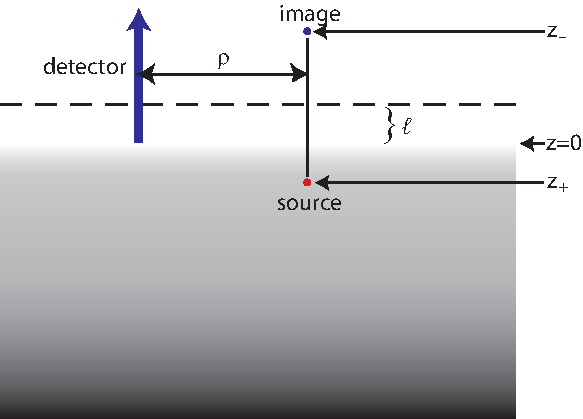
\includegraphics[width=11cm]{./figures/semiinfinite.pdf}
\caption{The semi-infinite case where the image method is used to find the solution.}
\label{semiinf}
\end{center}
\end{figure}
\subsubsection{Slab Geometry}
The solution for the slab geometry is just an expansion on the solution for the semi-infinite case. We use the method of images again. This time there is a second boundary located on the bottom, and we again make the assumption that $\Phi=0$ some distance $\ell$ away from the air-diffuse media interface on the bottom $z=L$ as well. As in the semi-infinite case, we add an image charge above the top boundary. But now we need to add another image below the bottom boundary to cancel our source on that side as well. In fact, we need to cancel the first image on the top across the bottom boundary too.
Now we need to account for these images with more images above the top boundary again!! Now you see that we can do this again and again... We start to see a pattern in the position of these sources and we can write the Green's function for the original source and all these images as an infinite sum:
\begin{figure}[htp]
\begin{center}
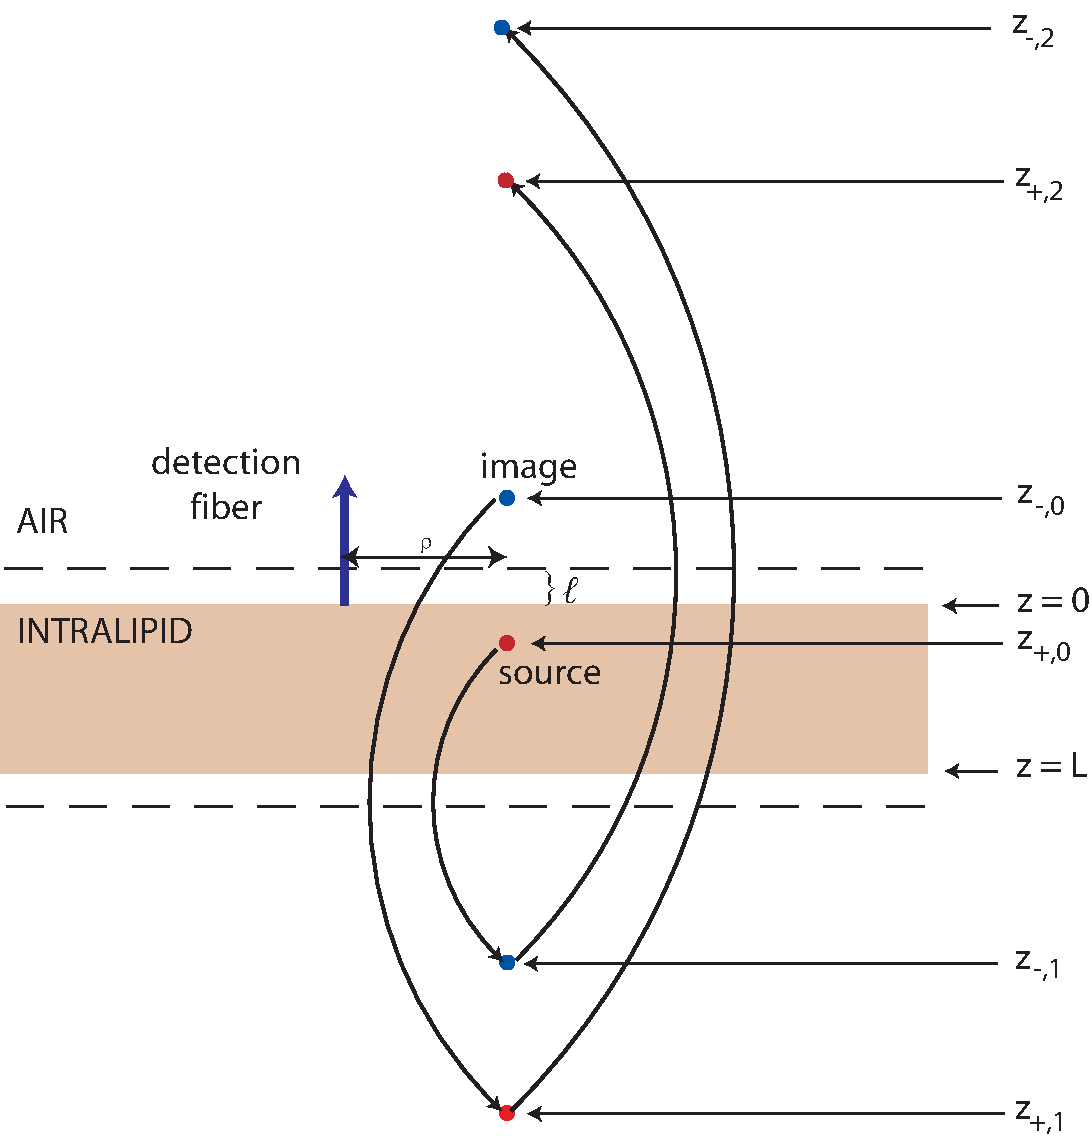
\includegraphics[width=9cm]{./figures/slab3.pdf}
\caption{The slab case where the image method is used again to find  the solution. This time since there are two boundaries, we have to sum over a larger number of source and sink images.}
\label{slab}
\end{center}
\end{figure}
\begin{equation}
G(\rho_s,z_s;\rho,z) = \frac{vS_{AC}}{4\pi D} \sum_{m=-\infty}^{m=\infty} 
\left\{ \frac{exp[ikr_{+,m}]}{r_{+,m}} - \frac{exp[ikr_{-,m}]}{r_{-,m}} \right\} \nonumber
\end{equation}
\begin{eqnarray}
\label{ext_both}
r_{+,m} = & \sqrt{(\rho-\rho_s)^2+(z-z_{+,m})^2} \nonumber \\
r_{-,m} = & \sqrt{(\rho-\rho_s)^2+(z-z_{-,m})^2}
\end{eqnarray}
\noindent
where $z_{+,m}=2m(L+2\ell)+z_s$, $z_{-,m}=2m(L+2\ell)-2\ell-z_s$, $m=0,\pm 1, \pm 2, ...$, and $L$ is the thickness of the slab. For the semi-infinite geometry, only the $m=0$ term is used. 
\subsection{Boundary Conditions}
In this section we will determine the value of $\ell$ that we used before for our semi-infinite and slab solutions. This derivation follows the approach of Haskell's paper \cite{Haskell1994}. We start by defining the radiance ($W/m^2sr^1$), which measures the amount of light passes through a given area within some solid angle in a specific direction. Integrating the radiance over all possible angles will give us the fluence rate that we've been using thus far. 
\begin{eqnarray}
\Phi({\bf r}) &=& \int\int_{4\pi} d\Omega \ L({\bf r},{\bf s})\\
{\bf j}({\bf r}) &=& \int\int_{4\pi} d\Omega \ L({\bf r},{\bf s}) \ {\bf s}
\end{eqnarray}
In the diffusion approximation, the radiance can be approximated by an isotropic fluence rate term plus an additional term for some small directional flux pointing along ${\bf s}$:
\begin{equation}
\label{Radiance}
L({\bf r},{\bf s}) = \frac{1}{4\pi} [ \Phi({\bf r}) + 3 {\bf j}({\bf
  r}) \cdot {\bf s}] \ .
\end{equation}
\begin{figure}[htp]
\begin{center}
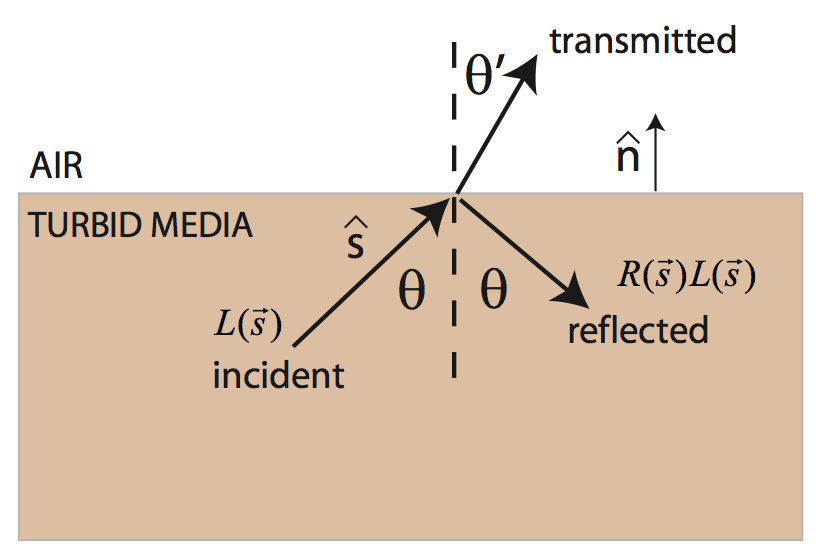
\includegraphics[width=7cm]{./figures/BoundaryReflect.png}
\caption{At the boundary, some of the incident light is Fresnel reflected back into the media due to index mismatch. This reflected light accounts for all of the light that is diffusing inwards towards the media at the boundary.}
\label{BoundaryReflect}
\end{center}
\end{figure}
Since we are interested in taking noninvasive measurements, we will look at the radiance at the air-tissue boundary. If ${\bf n}$ is the outward normal the tissue surface and ${\bf s}$ gives us the direction of the light propagation, then the fluence rate of the light exiting and entering the tissue is given by integrating $L({\bf s}) ({\bf s} \cdot {\bf n})$ over all outward directions and integrating  $L({\bf s}) ({\bf s} \cdot {- \bf n})$ over all inward directions
respectively. Air is not a scattering medium so there is no light entering the tissue from the boundary with the exception of the Fresnel reflected light of the outgoing light due to the index mismatch at the boundary. If $R({\bf \theta})$ is the Fresnel reflection coefficient for unpolarized light, then
\begin{equation}
\label{bc1}
\int\int_{{\bf s} \cdot {\bf n} > 0} R({\bf s}) L({\bf s}) ({\bf s} \cdot {\bf n}) d\Omega =
\int\int_{{\bf s} \cdot {\bf n} < 0} L({\bf s}) ({\bf s} \cdot {- \bf
  n}) d\Omega \ .
\end{equation}
\begin{equation}
\label{bc2}
\frac{1}{4\pi}\int\int_{{\bf s} \cdot {\bf n} > 0} R({\bf s}) [ \Phi({\bf
  r}) + 3 {\bf j}({\bf r}) \cdot {\bf s}] ({\bf s} \cdot {\bf n})
d\Omega = \frac{1}{4\pi} \int\int_{{\bf s} \cdot {\bf n} < 0} [ \Phi({\bf r}) + 3 {\bf j}({\bf
  r}) \cdot {\bf s}] ({\bf s} \cdot {-\bf n}) d\Omega \ .
\end{equation}
Changing into spherical coordinates, ${\bf s}\cdot{\bf
  n}=\cos\theta$ and ${\bf j}\cdot{\bf n}=j_z\cos\theta$, the integral
on the RHS then becomes
\begin{eqnarray}
\label{bc3}
\frac{1}{4\pi}\int\int_{{\bf s} \cdot {-\bf n}} [-\Phi\cos\theta +
3j_z\cos^2\theta]\sin\theta d \phi d\theta &=&
\frac{1}{4}\int_{\pi/2}^{\pi} [-\Phi\cos\theta +
3j_z\cos^2\theta]\sin\theta d\theta \nonumber\\ 
&=&\frac{1}{2}\int_{0}^{-1} [\Phi u - 3j_zu^2] du \nonumber \\
&=&\frac{\Phi}{4}+\frac{j_z}{2}
\end{eqnarray}
\noindent
where I have used $u=\cos\theta$ substitution to get the second line. Similarly, the integral on the LHS becomes 
\begin{eqnarray}
\label{bc4}
\frac{1}{4\pi}\int\int_{{\bf s} \cdot {\bf n}} R({\bf s})[\Phi\cos\theta -
3j_z\cos^2\theta]\sin\theta d \phi d\theta &=&  \frac{1}{4}\int_{0}^{\pi/2}
 R({\bf \theta})[\Phi\cos\theta - 3j_z\cos^2\theta]\sin\theta d\theta \nonumber\\
&=& \frac{1}{4}\Phi\int_{0}^{\pi/2}2R({\bf \theta})\cos\theta\sin\theta
d\theta - \nonumber \\
& & \frac{1}{2} j_z\int_{0}^{\pi/2}3R({\bf \theta})\cos^2\theta\sin\theta d\theta \nonumber \\
&=&\frac{\Phi}{4}R_\Phi-\frac{j_z}{2}R_j
\end{eqnarray}
\noindent
where we have defined
\begin{equation}
\label{Rj}
R_j = \int_0^{\pi/2} 2 sin \theta \ cos^2 \theta \ R(\theta) \ d\theta
\end{equation}
\begin{equation}
\label{Ru}
R_{\Phi} = \int_0^{\pi/2} 3 sin \theta \ cos \theta \ R(\theta) \ d\theta
\end{equation}
\noindent
and $R(\theta)$ are the Fresnel Reflection coefficients for which I give the expression below for unpolarized light.
\begin{equation}
R(\theta) = \left\{ \begin{array}{ll}
    \frac{1}{2}(\frac{n_{media}\cos\theta'-n_{air}\cos\theta}
                     {n_{media}\cos\theta'+n_{air}\cos\theta})^2 +
 \frac{1}{2}(\frac{n_{media}\cos\theta-n_{air}\cos\theta'}
                     {n_{media}\cos\theta+n_{air}\cos\theta'})^2 
      & \mbox{when $0 \leq \theta \leq \theta_c$} \\
    1 & \mbox{when $\theta_c \leq \theta \leq \pi /2$ }
    \end{array}
  \right.
\end{equation}
\noindent
Now plugging in equations \ref{bc3} and \ref{bc4} into equation \ref{bc1} we get
\begin{equation}
\label{bc2}
R_{\Phi}\frac{\Phi}{4} - R_j \frac{j_z}{2} = \frac{\Phi}{4} + \frac{j_z }{2}
\end{equation}
\\
We now introduce the effective reflection coefficient which we will
define as
\begin{equation}
R_{eff} = \frac{R_{\Phi} + R_j}{2 - R_{\Phi} + R_f} \
\end{equation}
\\
which simplifies equation \ref{bc2} to give us
\begin{equation}
\label{bc3}
R_{eff} \left( \frac{\Phi}{4} - \frac{j_z}{2} \right) = \frac{\Phi}{4} + \frac{j_z}{2} \ .
\end{equation}
\\
which shows us that $R_{eff}$ gives us the fraction of the radiance that is reflected. 

We can also determine the value of $R_{eff}$ experimentally. We start with the obvious statement that the reflectance and transmission accounts for all of the photons
\begin{equation}
  R + T = 1 \ .
\end{equation}
For diffuse media, we can relate the internal and external transmission ($T_{internal}, T_{external}$ based on Snell's law and conservation of energy (Orchard 1969)
\begin{equation}
  T_{internal} = T_{external} /n_{rel}^2
\end{equation}
where $n_{rel} = n_{medium}/n_{air}$ is the relative refractive index. Now we state that
\begin{equation}
\label{refinttoext}
R_{internal} = 1 - (1 - R_{external})/n_{rel}^2
\end{equation}
Egan (1979) \cite{Egan1979} did a power series curve fit to the external reflectance data tabulated by Orchard \cite{Orchard1969} to get
\begin{equation}
R_{external} = 0.440 + 0.710n_{rel} -0.332n_{rel}^2 + 0.0636n_{rel}^3
\end{equation}
From \ref{refintoext} we find that \cite{Sevick2002}
\begin{equation}
\label{exp eff}
R_{eff} = R_{internal} = -1.440n_{rel}^{-2} + 0.710n_{rel}^{-1} + 0.668 + 0.0636n_{rel}
\end{equation}
\noindent
We further simplifiy \ref{bc3} by using a relation known as Fick's rule which draws its name from its similarity to the equation describing ordinary gas diffusion.
\begin{equation}
j_z = -D \nabla \Phi \cdot {\bf z} \ ,
\end{equation}
\noindent
This is actually a basic relation that comes out of the diffusion approximation and comes out during the derivation of the diffusion equation from the radiative transport equation \cite{Case1967} to be covered in a later section. Using this relation, \ref{bc3} becomes
\begin{equation}
\label{bc4}
\Phi + \left[2D \frac{1+R_{eff}}{1-R_{eff}}\right] \nabla \Phi \cdot {\bf n} = 0 \ .
\end{equation}
or
\begin{equation}
\label{BC_DE}
\Phi + \ell\ \nabla \Phi\cdot{\bf n} = 0
\end{equation}
\\
\noindent
where we have replaced the terms inside the square bracket with $\ell$. From here we can use the Extrapolated-Boundary Condition \cite{Haskell1994, Aronson1993, Aronson1995} which states that the fluence rate drops lienarly to zero at the distance $\ell$ away from the boundary that we have worked out ($\Phi(\rho,z=-\ell) = 0$). Then we have the boundary we need to solve for the semi-infinite and slab geometries we covered earlier in the section.
\vspace{3mm}
{\bf [Side note about $R_{eff}$:}, note that we can also determine
the value of $R_{eff}$ experimentally. We do this by stating that the
reflectance and transmission accounts for all of the photons
\begin{equation}
  R + T = 1 \ .
\end{equation}
For diffuse media, we can relate the internal and external transmission ($T_{internal}, T_{external}$ based on Snell's law and
conservation of energy (Orchard 1969)
\begin{equation}
  T_{internal} = T_{external} /n_{rel}^2
\end{equation}
where $n_{rel} = n_{medium}/n_{air}$ is the relative refractive
index. Now we state that
\begin{equation}
\label{refinttoext}
R_{internal} = 1 - (1 - R_{external})/n_{rel}^2
\end{equation}
Egan (1979) \cite{Egan1979} did a power series curve fit to the external reflectance data tabulated by Orchard \cite{Orchard1969} to get
\begin{equation}
R_{external} = 0.440 + 0.710n_{rel} -0.332n_{rel}^2 + 0.0636n_{rel}^3
\end{equation}
From \ref{refinttoext} we find that \cite{Sevick2002}
\begin{equation}
\label{exp eff}
R_{eff} = R_{internal} = -1.440n_{rel}^{-2} + 0.710n_{rel}^{-1} + 0.668 + 0.0636n_{rel}
\end{equation}
Which is often the experimental value of the effective reflection coefficient often stated by our group {\bf ]}
\begin{figure}[h]
  \begin{center}
    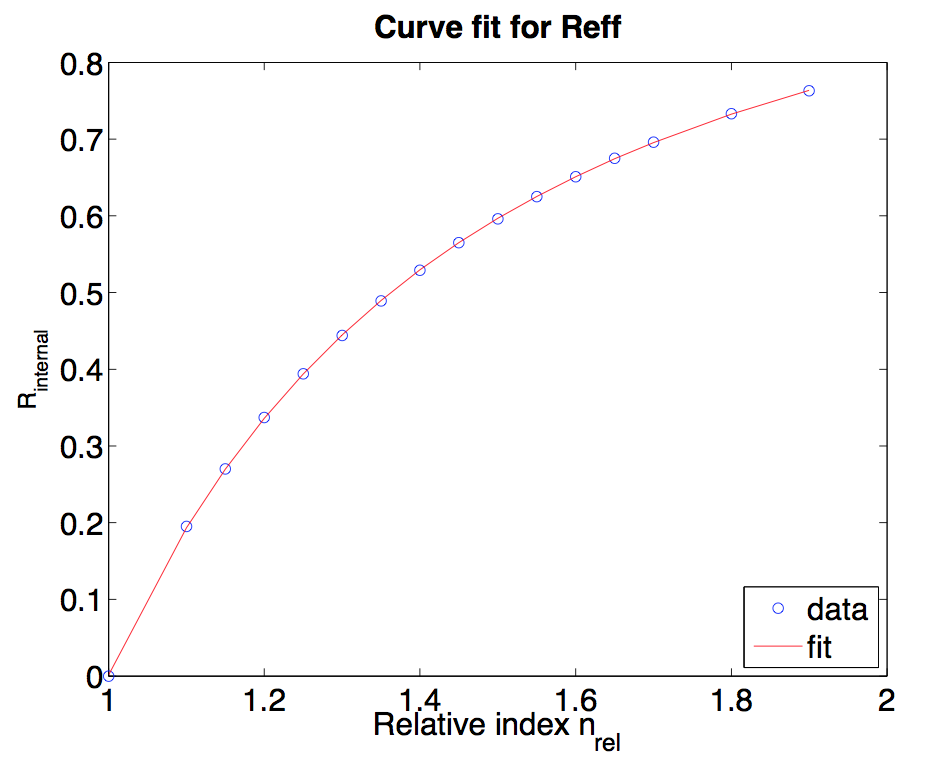
\includegraphics[scale=0.44]{./figures/ReflectanceCurveFit.png}
    \label{ReflectanceCurveFit}
    \caption{A plot showing the tabulated data taken by Orchard fitted with the power series given by Egan.} 
  \end{center}
\end{figure}



\section{Reconstruction Methods}
\subsection{Linear Reconstruction Methods}










\subsection{Nonlinear Reconstruction Methods}